% Created 2021-09-11 Sat 08:17
% Intended LaTeX compiler: xelatex
\documentclass[letterpaper]{article}
\usepackage{graphicx}
\usepackage{grffile}
\usepackage{longtable}
\usepackage{wrapfig}
\usepackage{rotating}
\usepackage[normalem]{ulem}
\usepackage{amsmath}
\usepackage{textcomp}
\usepackage{amssymb}
\usepackage{capt-of}
\usepackage{hyperref}
\usepackage[margin=1in]{geometry}
\usepackage{fontspec}
\usepackage{indentfirst}
\setmainfont[ItalicFont = LiberationSans-Italic, BoldFont = LiberationSans-Bold, BoldItalicFont = LiberationSans-BoldItalic]{LiberationSans}
\newfontfamily\NHLight[ItalicFont = LiberationSansNarrow-Italic, BoldFont       = LiberationSansNarrow-Bold, BoldItalicFont = LiberationSansNarrow-BoldItalic]{LiberationSansNarrow}
\newcommand\textrmlf[1]{{\NHLight#1}}
\newcommand\textitlf[1]{{\NHLight\itshape#1}}
\let\textbflf\textrm
\newcommand\textulf[1]{{\NHLight\bfseries#1}}
\newcommand\textuitlf[1]{{\NHLight\bfseries\itshape#1}}
\usepackage{fancyhdr}
\pagestyle{fancy}
\usepackage{titlesec}
\usepackage{titling}
\makeatletter
\lhead{\textbf{\@title}}
\makeatother
\rhead{\textrmlf{Compiled} \today}
\lfoot{\theauthor\ \textbullet \ \textbf{2021-2022}}
\cfoot{}
\rfoot{\textrmlf{Page} \thepage}
\titleformat{\section} {\Large} {\textrmlf{\thesection} {|}} {0.3em} {\textbf}
\titleformat{\subsection} {\large} {\textrmlf{\thesubsection} {|}} {0.2em} {\textbf}
\titleformat{\subsubsection} {\large} {\textrmlf{\thesubsubsection} {|}} {0.1em} {\textbf}
\setlength{\parskip}{0.45em}
\renewcommand\maketitle{}
\author{Houjun Liu}
\date{\today}
\title{Bio-Molecules Quiz Review}
\hypersetup{
 pdfauthor={Houjun Liu},
 pdftitle={Bio-Molecules Quiz Review},
 pdfkeywords={},
 pdfsubject={},
 pdfcreator={Emacs 27.2 (Org mode 9.4.4)}, 
 pdflang={English}}
\begin{document}

\maketitle


\section{Bio-Molecules Quiz Review}
\label{sec:org45f09f3}
\subsection{Paul's Review Sheet}
\label{sec:org1fb11cd}
\href{https://docs.google.com/document/d/1wGN3RNZCN-hkP2gJe2C7FHGZi\_-YfCE6aJCZy-0N53s/edit}{\ldots{}
is here}

And Jack's raw answers:
\href{KBhBIO201BioMoleculesRAW.org}{KBhBIO201BioMoleculesRAW}

\subsection{Jack's Review Smanza}
\label{sec:org2501c95}
\begin{itemize}
\item \textbf{Macromolecules}

\begin{itemize}
\item \href{KBhBIO101Carbs.org}{KBhBIO101Carbs} \&
\href{KBhBIO101StructuresofCarbs.org}{KBhBIO101StructuresofCarbs}
\item \href{KBhBIO101Lipids.org}{KBhBIO101Lipids} \&
\href{KBhBIO101StructuresOfLipids.org}{KBhBIO101StructuresOfLipids}
\end{itemize}

\item \textbf{Proteins, Amino Acids, and Enzymes}

\begin{itemize}
\item \href{KBhBIO101AminoAcids.org}{KBhBIO101AminoAcids} \&
\href{KBhBIO101FunctionalGroups.org}{KBhBIO101FunctionalGroups}
\item \href{KBhBIO101Proteins.org}{KBhBIO101Proteins}
\item \href{KBhBIO101Enzymes.org}{KBhBIO101Enzymes}
\end{itemize}

\item \textbf{Cell Structure, Type, and Transport}

\begin{itemize}
\item \href{KBhBIO101Cells.org}{KBhBIO101Cells}. Duh.
\item \href{KBhBIO101CellMembraines.org}{KBhBIO101CellMembraines}
\item \href{KbhBIO101CellTransport.org}{KbhBIO101CellTransport}
\item \href{KBhBIO101EukaryoticOrganells.org}{KBhBIO101EukaryoticOrganells}
\begin{itemize}
\item 
\end{itemize}
\href{KBhBIO101OrganellsBasedOnMembranes.org}{KBhBIO101OrganellsBasedOnMembranes}
\end{itemize}
\end{itemize}

\subsection{Helpful review items}
\label{sec:org045f3ae}
\begin{figure}[htbp]
\centering
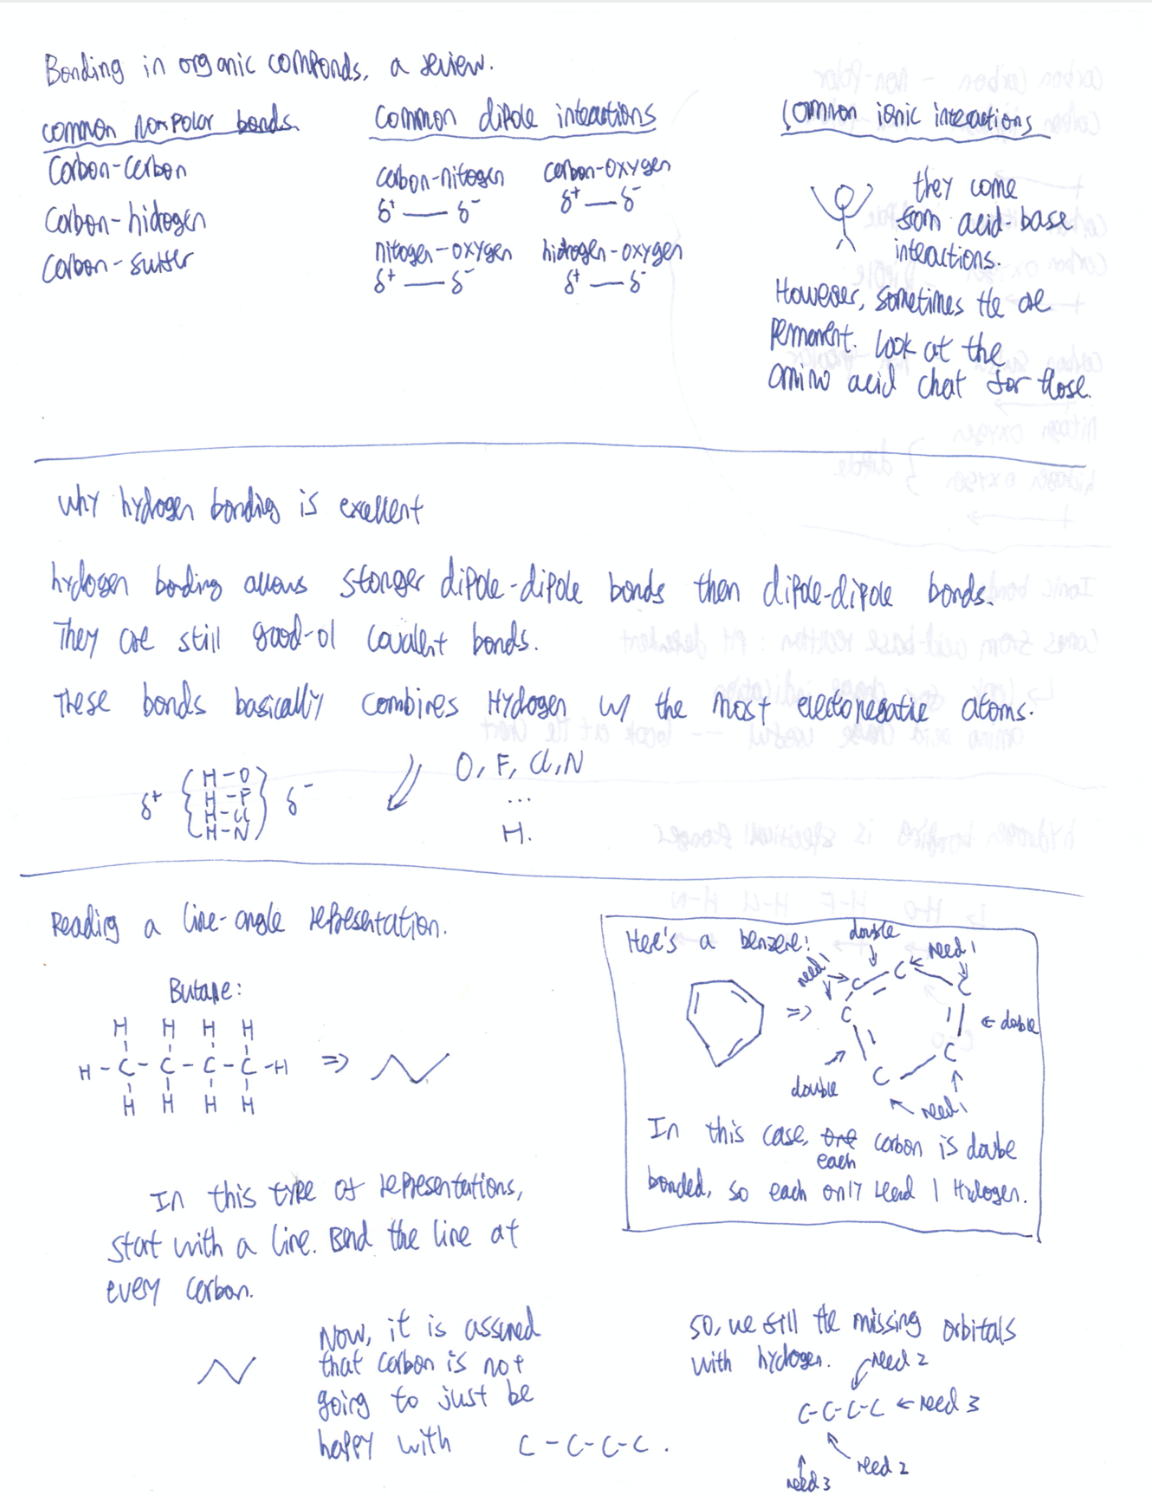
\includegraphics[width=.9\linewidth]{Screen Shot 2020-10-09 at 11.58.55 AM.png}
\caption{Screen Shot 2020-10-09 at 11.58.55 AM.png}
\end{figure}

\begin{figure}[htbp]
\centering
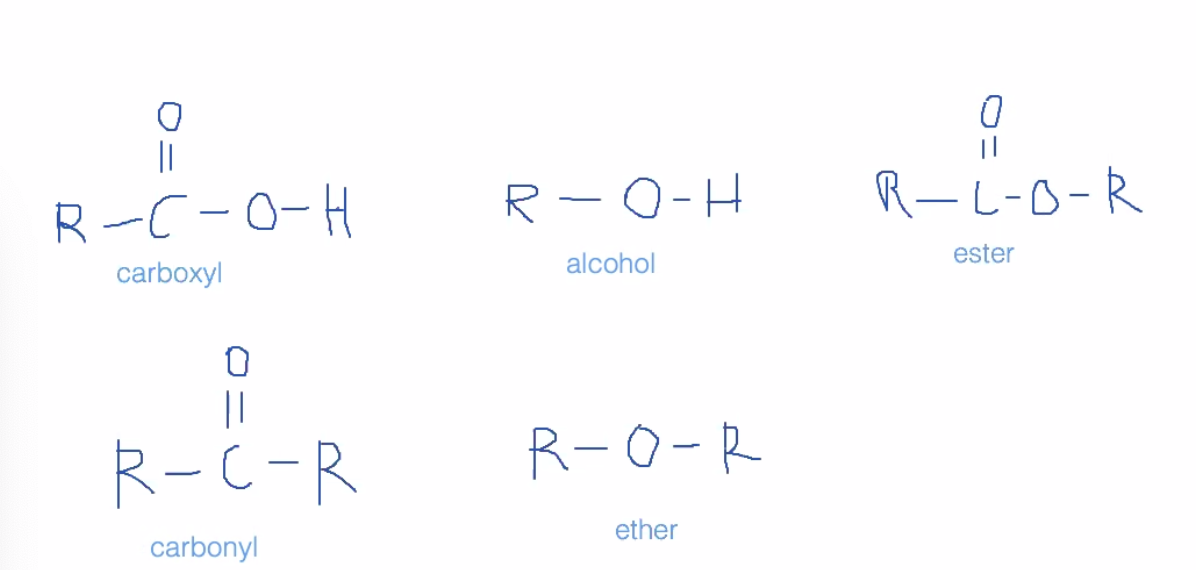
\includegraphics[width=.9\linewidth]{Screen Shot 2020-10-12 at 2.34.16 PM.png}
\caption{Screen Shot 2020-10-12 at 2.34.16 PM.png}
\end{figure}
\end{document}
